%==============================================================================
% VidTrust AI -- IEEE conference paper, DRAFT
%
% Compiles as-is on Overleaf (IEEEtran ships with it). Needs the three figures
% produced by make_figures.py in the same directory.
%
% DRAFT NOTES -- resolve before submission, see paper/README.md:
%   * confirm the author list, roll numbers and whether the guide is a co-author
%   * verify every reference against the published record (pages, DOI, year)
%   * pick a venue; the abstract length limit and page limit follow from it
% Every numeric result below is reproducible from a script in this repository;
% the command for each one is named in Section VI-A.
%==============================================================================
\documentclass[conference]{IEEEtran}
\IEEEoverridecommandlockouts

\usepackage{cite}
\usepackage{amsmath,amssymb}
\usepackage{graphicx}
\usepackage{booktabs}
\usepackage{array}
\usepackage{url}

% HuggingFace model identifiers are long, unbroken strings containing slashes,
% hyphens and underscores, and they overflow an IEEE column if set as ordinary
% \texttt. \path sets them verbatim (so underscores need no escaping) and the
% break list below lets them wrap, which keeps the full identifier in the table
% rather than an abbreviation.
\urlstyle{tt}
\def\UrlBreaks{\do\/\do\-\do\_\do\.}
\def\UrlBigBreaks{\do\/}
\newcommand{\hfid}[1]{\path{#1}}
\usepackage[hidelinks]{hyperref}
\usepackage[T1]{fontenc}

\def\BibTeX{{\rm B\kern-.05em{\sc i\kern-.025em b}\kern-.08em
    T\kern-.1667em\lower.7ex\hbox{E}\kern-.125emX}}

\begin{document}

\title{Availability-Aware Multi-Signal Fusion for\\Detecting Machine-Generated Images and Video}

\author{
\IEEEauthorblockN{Dhruv Saraf, Om Mahajan, Arjun Patil, Yash Mahajan}
\IEEEauthorblockA{\textit{Department of Information Technology} \\
\textit{K.\,J.\ Somaiya College of Engineering} \\
\textit{Somaiya Vidyavihar University}, Mumbai, India}
\and
\IEEEauthorblockN{Dr.\ Sanjay Vidhani}
\IEEEauthorblockA{\textit{Department of Information Technology} \\
\textit{K.\,J.\ Somaiya College of Engineering} \\
\textit{Somaiya Vidyavihar University}, Mumbai, India}
}

\maketitle

\begin{abstract}
Fully synthetic images and video are now produced by hundreds of publicly
available generators, and a detector that relies on any single cue fails
whenever that cue is absent. We present VidTrust~AI, a detector that fuses
three deliberately independent signals: a pretrained neural classifier,
provenance metadata (EXIF/XMP/C2PA), and a fast Fourier transform (FFT)
high-frequency energy ratio. They are combined by an
\emph{availability-aware} fusion rule, under which a signal that cannot run
is removed from the weighted average and the remaining weights are
renormalised, rather than being scored as zero. On a
400-image balanced subset of Community Forensics spanning 50 generators, the
fused system reaches ROC-AUC 0.9196, against 0.8397 for the classifier alone
and 0.9012 for the frequency signal alone. We further show that the standard
evaluation protocol conflates synthesis artefacts with resampling history:
under a centre-crop control that equalises processing history without
interpolation, AUC rises to 0.9487 while recall is unchanged to four decimal
places; the entire gain is a reduction in false positives on real
photographs, from 70 to 39. We report two negative results that only
per-signal logging exposed: a three-character provenance signature that fired
at full confidence on 62 of 200 real photographs, and an earlier classifier
under which the fused ensemble ranked \emph{below} its lowest-weighted
component. Finally, we measure an operating point that improves held-out
accuracy from 0.8342 to 0.9664 and decline to adopt it, because it is fitted
to a dataset confound we can name. We argue that per-signal score dumping and
ablation should be treated as a minimum reporting standard for fused
detectors.
\end{abstract}

\begin{IEEEkeywords}
synthetic media detection, AI-generated image detection, sensor fusion,
content provenance, C2PA, ablation study, evaluation methodology
\end{IEEEkeywords}

%==============================================================================
\section{Introduction}
%==============================================================================

The manipulated media that most needs checking is no longer a face swapped
into an otherwise genuine photograph. It is media that is synthetic in its
entirety: an image or clip that no camera ever recorded. Latent diffusion
models~\cite{rombach2022} and their thousands of community fine-tunes have
made such media cheap, and the detection problem has shifted with it. A
face-swap detector~\cite{rossler2019} needs an original to compare against; a
fully synthetic image has no original, and frequently no photographed face at
all.

Detectors for this problem are commonly single-model
classifiers~\cite{wang2020,ojha2023,corvi2023}. That design has a structural
weakness that is easy to miss in benchmark numbers: it has exactly one way to
be wrong, and nothing to check it against. An ensemble of independent signals
can in principle cover that gap, but only if it handles the case that
motivates it. Provenance metadata is the strongest available evidence of
synthetic origin when it is present, and it is absent from the great majority
of media in circulation, because every social platform re-encodes on upload
and strips it. A fusion rule that scores a missing signal as $0.0$ treats
``no evidence'' as ``evidence of authenticity'' and pushes every stripped file
toward a verdict of real.

This paper makes four contributions.

\begin{enumerate}
\item \textbf{An availability-aware fusion rule} (Section~\ref{sec:fusion})
  under which an inoperative signal is excluded from the weighted average and
  the remaining weights renormalised, with total signal failure mapping to
  maximum ignorance rather than to either verdict.
\item \textbf{A two-track evaluation protocol} (Section~\ref{sec:method}) that
  refuses to average a large public set on which the provenance signal is
  structurally dead with a small hand-collected set on which it is the only
  thing being tested.
\item \textbf{A resolution-normalisation control} (Section~\ref{sec:normal})
  showing that a naive protocol on the standard public set measures
  resampling history in addition to synthesis, and quantifying how much of
  the reported performance that accounts for.
\item \textbf{Two reported negative results} (Section~\ref{sec:findings}) that
  were invisible to unit tests and to aggregate metrics, and were surfaced
  only because the evaluation harness dumps every signal's score and
  availability flag per file.
\end{enumerate}

We state at the outset what this work does not claim. No model is trained or
fine-tuned here; the classifier is used exactly as published. The fusion
weights and verdict thresholds are hand-chosen and remain unfitted, and
Section~\ref{sec:thresholds} reports a measured operating point that we
deliberately did not adopt. The evaluation set has content and resolution
confounds that we characterise rather than remove, so the absolute figures
below are an upper bound on field performance, not an estimate of it.

%==============================================================================
\section{Related Work}
%==============================================================================

\textbf{Learned detectors.} Wang~et~al.~\cite{wang2020} showed that a
classifier trained on the output of a single CNN generator transfers
surprisingly well across architectures, establishing the single-classifier
baseline that most subsequent work follows.
Gragnaniello~et~al.~\cite{gragnaniello2021} re-examined those claims under
realistic post-processing and found the reported robustness substantially
overstated once compression and resizing are applied. For diffusion output
specifically, Corvi~et~al.~\cite{corvi2023} showed that detectors trained on
GAN imagery degrade sharply, and Ojha~et~al.~\cite{ojha2023} argued for
features not tied to one generator family. Our classifier signal is an
off-the-shelf instance of this line of work, and Section~\ref{sec:selection}
shows why the specific instance matters more than the surrounding
architecture.

\textbf{Frequency-domain cues.} Up-sampling layers in generative
architectures leave periodic spectral artefacts, which Durall~et~al.\
\cite{durall2020} and Frank~et~al.~\cite{frank2020} exploited directly. These
cues are strong on the generators they were characterised on and known to be
fragile under compression and rescaling. We include a deliberately simple
FFT-based statistic as an independent, fully explainable signal, and
Section~\ref{sec:limits} reports the evidence that it is not yet measuring
synthesis.

\textbf{Provenance.} The C2PA specification~\cite{c2pa} defines
cryptographically signed content credentials that travel inside the file.
Provenance is qualitatively different from the other two signals: it is
evidence about the file's history rather than an inference from its pixels,
and it is high-precision and low-recall by construction. The literature
treats detection and provenance largely separately; combining them raises the
availability problem that motivates this paper.

\textbf{Evaluation practice.} Our protocol follows the concern raised in
\cite{gragnaniello2021} that detector evaluations frequently measure dataset
artefacts. Community Forensics~\cite{park2025} supplies per-image generator
attribution, which makes per-generator failure analysis possible rather than
merely aggregate.

%==============================================================================
\section{System Design}
%==============================================================================

Fig.~\ref{fig:arch} gives the pipeline. The system exposes an HTTP API; a
single endpoint accepts an image or a video and returns a verdict, a fused
confidence, and the full per-signal breakdown that produced it.

\begin{figure*}[t]
\centering
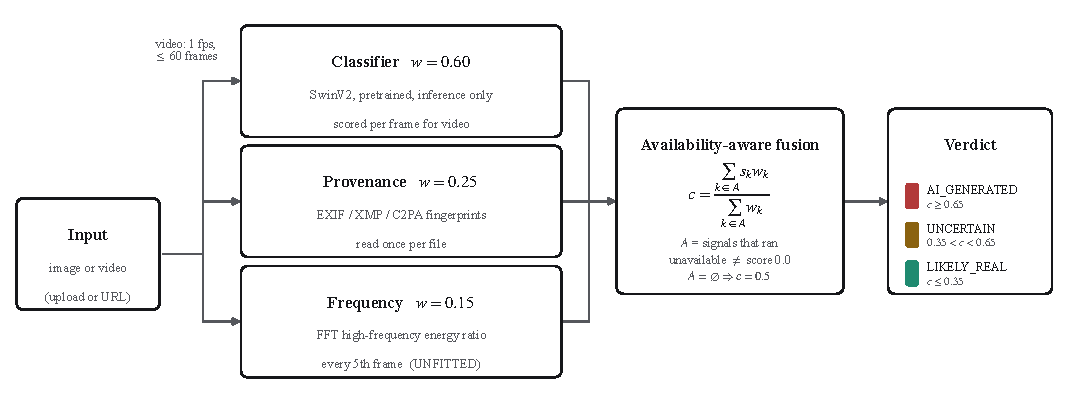
\includegraphics[width=\textwidth]{fig1_architecture.pdf}
\caption{Pipeline. Three independent signals are computed, then fused over
only those that actually ran. Video is treated as images over time: frames are
sampled at 1\,fps up to a 60-frame cap, the classifier scores every sampled
frame, provenance is read once from the container, and the frequency signal
runs on every fifth frame.}
\label{fig:arch}
\end{figure*}

\subsection{The three signals}

\textbf{Classifier ($w=0.60$).} A pretrained image-classification head is
applied to the image, or to every sampled frame of a video, and its label
distribution is collapsed into $P(\text{machine-generated})$. Label
vocabularies are mapped explicitly; a head reporting only generic labels such
as \texttt{LABEL\_0}/\texttt{LABEL\_1} is \emph{not} mapped by guessing an
index, because a wrong guess silently inverts the signal. An unrecognised
vocabulary makes the signal report unavailable. The model used in all
experiments below is a SwinV2~\cite{liu2022} head
(\texttt{haywoodsloan/ai-image-detector-deploy}, 744\,MB) selected by
measurement in Section~\ref{sec:selection}. It is loaded once at application
start-up and never on the request path.

\textbf{Provenance ($w=0.25$).} The file is inspected for two opposite kinds
of evidence. A generator fingerprint (a known generator name in decoded EXIF
or XMP text, or a C2PA/JUMBF manifest marker) yields score 1.0. Genuine
camera EXIF (\texttt{Make} and \texttt{Model} present, no generator string)
yields 0.0. A file carrying neither makes the signal report
\emph{unavailable}, which is the case that Section~\ref{sec:fusion} exists to
handle. Manifest detection is a bounded raw-byte scan for markers rather than
a full C2PA parse, so the system can report that a manifest is present but not
who signed it; this is a stated implementation gap.

\textbf{Frequency ($w=0.15$).} The image is converted to greyscale, resized to
$512\times512$, and its DC component removed. The 2-D FFT is taken, and the
fraction of total spectral energy lying outside a central low-frequency disc
of radius $0.03125 \times 512 = 16$\,px is computed. That ratio is mapped
linearly onto $[0,1]$ over the interval $[0.05, 0.45]$. \textbf{Both endpoints
are unfitted}: they bracket the range over which the ratio moves at all, and
encode no measured boundary between generated and real. Section~\ref{sec:limits}
reports the calibration measurement that keeps them labelled that way.

The three signals were chosen to be independent in the \emph{evidence} they
consult (a neural judgement about pixels, a document-metadata lookup, and a
spectral statistic), so that they can disagree, and so that a failure mode of
one is not automatically a failure mode of another.

\subsection{Availability-aware fusion}
\label{sec:fusion}

Let $S=\{\text{model},\text{metadata},\text{frequency}\}$ with fixed weights
$w_k$, and let $A \subseteq S$ be the subset of signals that successfully
produced a score for this file. The fused confidence is
\begin{equation}
c \;=\; \frac{\sum_{k \in A} s_k w_k}{\sum_{k \in A} w_k},
\qquad
c \;=\; 0.5 \quad\text{if } A = \varnothing .
\label{eq:fuse}
\end{equation}

Equation~\eqref{eq:fuse} is a weighted average over the available signals with
the weights renormalised, not over all signals with missing ones zeroed. The
distinction is the central design decision of the system. A score of $0.0$
means ``this looks real''; unavailability means ``no evidence either way''.
Conflating them makes every file whose metadata was stripped drift toward a
verdict of authentic, and stripping metadata is exactly what every social
platform does on upload. Concretely, when provenance is absent the classifier
and frequency weights rescale from $0.60/0.15$ to $0.80/0.20$ and decide
between themselves.

The $A=\varnothing$ case maps to $0.5$ rather than to $0$: total signal
failure is maximum ignorance, and $0.5$ falls inside the abstention band
below, so a fully degraded system declines to answer instead of reporting
``real''.

The verdict is a three-way thresholding of $c$:
$c \ge 0.65 \Rightarrow$ \texttt{AI\_GENERATED};
$c \le 0.35 \Rightarrow$ \texttt{LIKELY\_REAL};
otherwise \texttt{UNCERTAIN}. \texttt{UNCERTAIN} is a first-class outcome. It
is the system declining to answer, and throughout this paper it is counted
separately from correct and incorrect rather than forced into a confusion
matrix.

\subsection{Degradation behaviour}

A failure of the classifier, the heaviest signal, is not an error response.
The signal reports unavailable, \eqref{eq:fuse} renormalises, and the other
two still produce a verdict. This follows from the same principle as the
fusion rule: a partial answer with its provenance visible is more useful than
no answer. The classifier's health is exposed on a separate status endpoint
rather than by failing analysis requests.

%==============================================================================
\section{Evaluation Methodology}
\label{sec:method}
%==============================================================================

\subsection{Two tracks, never averaged}

\textbf{Track A (public).} 400 images drawn from Community
Forensics~\cite{park2025} (CC~BY-NC-SA~4.0): 200 generated and 200 real. The
generated half spans 50 distinct generators at 4 images each, all of the
\texttt{LatDiff} architecture family; the real half is FFHQ~\cite{karras2019}.

\textbf{Track B (hand-collected).} 16 files, 13 labelled (4 generated, 9
real), collected by the authors: camera originals with intact EXIF, images
exported from commercial generators with Content Credentials, and files
deliberately routed through a messaging platform so that their metadata is
stripped in transit.

The tracks are never averaged, for a structural reason. Public datasets are
redistributed re-encoded: \textbf{0 of the 400 Track~A images carry any EXIF},
so the provenance signal cannot fire on a single one of them. Averaging would
let 400 images with a structurally dead signal drown 13 that exercise it, and
the resulting ``ensemble'' headline would silently be a two-signal result.
Track~A measures the classifier and frequency signals at scale; Track~B is the
only place provenance does anything at all.

Track~B carries a second disclosure. The 12 labelled images in it were the set
used to select the classifier (Section~\ref{sec:selection}). It is therefore
the model-selection set as well as the demonstration set, and its results are
reported as counts and as a functional check on the provenance branches,
never as an accuracy estimate.

\subsection{Metrics and the treatment of abstention}

Accuracy, precision, recall and $F_1$ are computed over \emph{decided} files
only, with abstentions excluded and reported separately as coverage
(decided/labelled). A detector that abstains on half the set and is right on
the rest is not accurate, and coverage is the honest companion to any accuracy
figure. ROC-AUC is computed over all labelled files including abstentions,
since AUC ranks a continuous score and never consults a threshold; it is
obtained through the rank (Mann--Whitney~$U$) identity with ties averaged.

\subsection{Threshold selection protocol}

Thresholds are chosen on one half of Track~A and reported on the other, split
stratified by class and seeded. A threshold picked on the same rows it is then
scored against is fitted to those rows and the resulting number estimates
nothing. This was not a formality: in an earlier configuration, a search over
all 400 rows at once suggested a cut near 0.06 lifting accuracy to roughly
0.73, while under a proper split the selection half chose 0.806 and reached
only 0.6850 held out.

\subsection{Resolution normalisation}
\label{sec:normal}

Every image in Track~A is analysed twice: as distributed (\emph{naive}), and
after a control we call \emph{resolution normalisation}.

The confound is this. Real images in this set are natively $1024\times1024$
and generated images natively $512\times512$, with no overlap. Every detector
in the pipeline resizes to 512 internally, so under the naive protocol the
real images arrive having been downsampled, which destroys high-frequency
content, while the generated images arrive untouched. A frequency statistic
can then separate the classes by measuring who was downsampled rather than who
was synthesised.

Resizing everything to a common target does \emph{not} fix this. A $1024^2$
image resized to 512 is still downsampled $2\times$ while a native $512^2$
image is not; the operation is identical but its effect depends on the input
size, which is exactly the variable that differs by class. We instead take a
\textbf{centre crop of $512\times512$ native pixels}. Nothing is interpolated,
no frequency content is created or destroyed, and every image reaches the
detectors as an unresampled $512\times512$ block, so the processing history is
genuinely identical across classes. Crops are written losslessly as PNG so the
control itself introduces no compression artefacts.

What the crop does not fix: it shows a sub-region of a large image and the
whole of a small one, so framing still differs. That is a content difference,
not a resampling one, and it is reported as such. Normalisation is refused on
Track~B, because re-saving as PNG discards the EXIF that Track~B exists to
test.

%==============================================================================
\section{Results}
%==============================================================================

\subsection{Classifier selection is a measurement, not a model-card decision}
\label{sec:selection}

The classifier was initially an SDXL-specific detector chosen from its model
card. Measured on the 12 labelled hand-collected images it was not merely weak
but \emph{anti-correlated}: mean score 0.438 on generated images against 0.574
on real photographs. It scored genuine iPhone originals at 0.998 ``artificial''
and a commercially generated image at 0.003. No weight and no threshold can
repair a signal that points the wrong way.

Five cached candidates were then scored over the identical files, inference
only (Table~\ref{tab:models}). The separation between the best and worst is
far larger than any fusion parameter could compensate for, which is the
practical lesson: for a fused detector, the choice of the heaviest component
dominates the choice of how to combine it.

\begin{table}[t]
\caption{Candidate classifiers on the 12 labelled hand-collected images
(4 generated, 8 real). Inference only; no fine-tuning.}
\label{tab:models}
\centering
\footnotesize
\begin{tabular}{@{}>{\raggedright\arraybackslash}p{1.52in}ccc@{}}
\toprule
Model (HuggingFace identifier) & Correct & Mean, gen. & Mean, real \\
\midrule
\hfid{haywoodsloan/ai-image-detector-deploy}     & 12/12 & 0.987 & 0.002 \\
\hfid{Ateeqq/ai-vs-human-image-detector}         & 11/12 & 0.752 & 0.001 \\
\hfid{dima806/ai_vs_human_generated_image_detection} & 8/12 & 0.012 & 0.011 \\
\hfid{Organika/sdxl-detector}                    &  5/12 & 0.438 & 0.574 \\
\hfid{dima806/ai_vs_real_image_detection}        &  4/12 & 0.766 & 0.694 \\
\bottomrule
\end{tabular}
\end{table}

\subsection{Track A headline}

Table~\ref{tab:headline} gives the aggregate results in both conditions and
Fig.~\ref{fig:roc} the corresponding ROC curves.

\begin{table}[t]
\caption{Track A, $n=400$. Metrics over decided files; coverage is
decided/labelled. AUC over all labelled files.}
\label{tab:headline}
\centering
\small
\begin{tabular}{@{}lcc@{}}
\toprule
 & naive & normalised \\
\midrule
Accuracy    & 0.7595 & \textbf{0.8384} \\
Precision   & 0.7107 & \textbf{0.8152} \\
Recall      & 0.8731 & 0.8731 \\
$F_1$       & 0.7836 & \textbf{0.8431} \\
ROC-AUC     & 0.9196 & \textbf{0.9487} \\
Coverage    & 0.9875 & 0.9900 \\
Abstentions & 5 & 4 \\
\midrule
True positives  & 172 & 172 \\
False positives & 70  & \textbf{39} \\
True negatives  & 128 & 160 \\
False negatives & 25  & 25 \\
\bottomrule
\end{tabular}
\end{table}

\begin{figure*}[t]
\centering
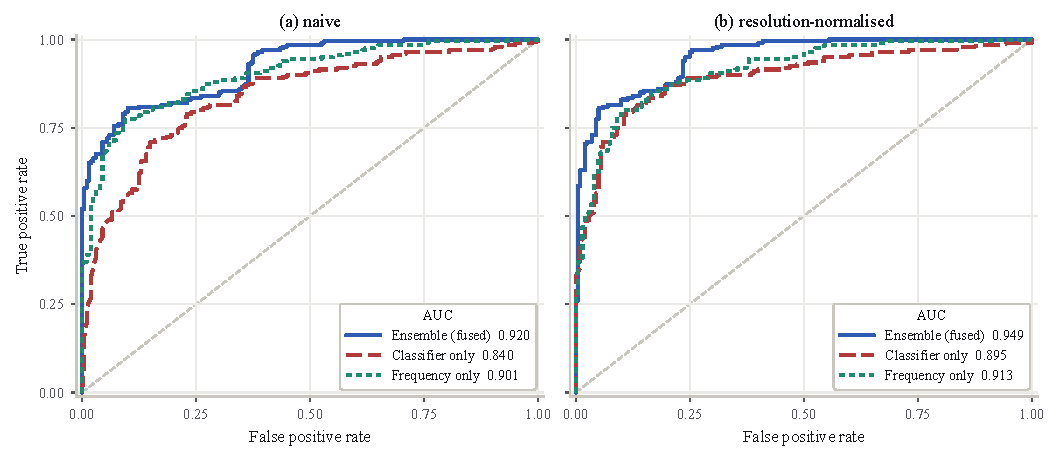
\includegraphics[width=\textwidth]{fig2_roc.pdf}
\caption{ROC curves on Track A, $n=400$, for the fused confidence and for two
of its constituents taken alone. The provenance signal is omitted: it is
unavailable on all 400 files and is a constant predictor here. The fused
ensemble dominates both constituents in both conditions.}
\label{fig:roc}
\end{figure*}

\textbf{Recall is identical in both conditions, to four decimal places}, and
that is not a coincidence. The generated images are natively $512^2$, so the
centre crop is a no-op on them: their per-image classifier and frequency
scores are byte-identical across the two runs. Only the real images change.
The entire normalised gain is therefore 31 fewer false positives on real
photographs (70$\rightarrow$39), which is exactly what removing a resampling
confound should do if that confound was inflating the real side.
Fig.~\ref{fig:normal} shows this directly: the two generated score
distributions coincide exactly while the real distribution shifts toward zero.

\begin{figure}[t]
\centering
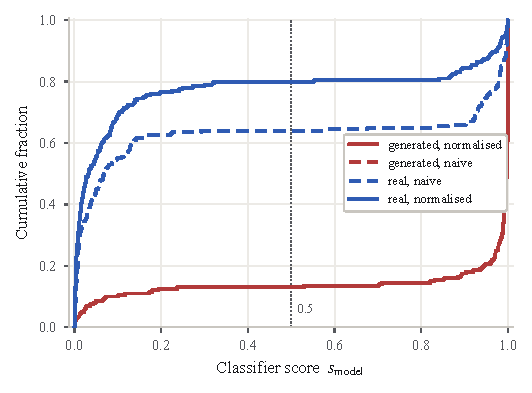
\includegraphics[width=\columnwidth]{fig3_normalisation.pdf}
\caption{Empirical CDF of the classifier score by class and condition,
Track~A. The two generated curves coincide exactly, because the centre crop
does not touch a natively $512\times512$ image, while the real distribution
moves toward zero under normalisation. The fraction of real images scoring above 0.5
falls from 72/200 to 40/200.}
\label{fig:normal}
\end{figure}

The system's characteristic error is calling a real FFHQ portrait generated,
not letting a generated image pass: precision (0.8152) trails recall (0.8731)
in the normalised condition.

\subsection{Ablation}

Table~\ref{tab:ablation} re-fuses the dumped per-signal scores under six
configurations. No inference is re-run: dropping a signal from a configuration
is arithmetically the same operation as that signal being unavailable at
runtime, so the ablation exercises the real fusion path rather than a parallel
reimplementation of it.

\begin{table}[t]
\caption{Ablation on Track A, recomputed from the per-signal dump. Rows marked
$\dagger$ are arithmetic identities forced by the dataset, not independent
results.}
\label{tab:ablation}
\centering
\small
\begin{tabular}{@{}lcccc@{}}
\toprule
& \multicolumn{2}{c}{naive} & \multicolumn{2}{c}{normalised} \\
\cmidrule(lr){2-3}\cmidrule(lr){4-5}
Configuration & Acc. & AUC & Acc. & AUC \\
\midrule
Full ensemble          & 0.7595 & \textbf{0.9196} & 0.8384 & \textbf{0.9487} \\
Classifier only        & 0.7563 & 0.8397 & 0.8367 & 0.8947 \\
Provenance only        & n/a    & 0.5000 & n/a    & 0.5000 \\
Frequency only         & 0.7194 & 0.9012 & 0.7177 & 0.9129 \\
$-$ Provenance$^\dagger$ & 0.7595 & 0.9196 & 0.8384 & 0.9487 \\
$-$ Frequency$^\dagger$  & 0.7563 & 0.8397 & 0.8367 & 0.8947 \\
\bottomrule
\end{tabular}
\end{table}

Three points must be read off this table carefully.

\textbf{The six rows contain only three distinct results.} Because provenance
is available on 0 of 400 files, ``ensemble $-$ provenance'' is arithmetically
identical to the full ensemble, and ``ensemble $-$ frequency'' is identical to
classifier-only. These are identities forced by the dataset and must not be
presented as independent findings. They are also the clearest possible
argument for why Track~B exists.

\textbf{The provenance row is not a measurement.} With no signal available
every image abstains, so accuracy, precision, recall and $F_1$ are undefined,
and the AUC of 0.5000 is the definition of a constant predictor.

\textbf{The frequency signal is extremely lopsided}: precision 1.0000 at
recall 0.3237 in both conditions. It never produces a false positive on this
set and catches roughly a third of generated images, the profile of a signal
that fires confidently on a visually distinct subset rather than one that
generalises.

\subsection{Threshold selection}
\label{sec:thresholds}

Table~\ref{tab:thresh} reports operating points chosen on the selection half
and scored on the held-out half.

\begin{table}[t]
\caption{Threshold selection, Track A. Chosen on one stratified half
($n=200$), reported on the other ($n=200$). Neither measured operating point
was adopted.}
\label{tab:thresh}
\centering
\small
\begin{tabular}{@{}llccc@{}}
\toprule
Cond. & Operating point & Sel. acc. & \textbf{Held-out} & Cov. \\
\midrule
naive & single cut 0.808      & 0.8350 & 0.8650 & 1.000 \\
naive & band 0.14\,/\,0.82    & 0.9220 & 0.9444 & 0.720 \\
naive & \emph{current} 0.35\,/\,0.65 & n/a & 0.7437 & 0.995 \\
norm. & single cut 0.808      & 0.8700 & 0.8800 & 1.000 \\
norm. & band 0.10\,/\,0.82    & 0.9586 & \textbf{0.9664} & 0.745 \\
norm. & \emph{current} 0.35\,/\,0.65 & n/a & 0.8342 & 0.995 \\
\bottomrule
\end{tabular}
\end{table}

Both measured operating points survive the selection/reporting split, and
neither was adopted. The band improves held-out accuracy from 0.8342 to 0.9664
but costs 25 points of coverage, abstaining on a quarter of inputs instead of
one in two hundred. That is a different product, not a tuned one. The single
cut is the more uncomfortable result: it improves held-out accuracy at
\emph{no} coverage cost, and says plainly that the hand-chosen 0.65 threshold
sits too low for this classifier's score distribution, because the real
portraits it is unsure about fuse into the 0.65--0.80 range and are called
generated.

We declined both because they are fitted to a score distribution shaped by the
dataset confounds of Section~\ref{sec:limits} (face photographs versus
digital art), which is not what the intended inputs look like, and because on
the 13 hand-collected files the current band makes no error. There is
therefore evidence that the threshold is wrong \emph{on FFHQ}, and no field
evidence that it is wrong in general. Adopting it would trade a measurable
gain on a confounded set for unknown behaviour on real inputs. The finding is
recorded; the constants are unchanged.

\subsection{Per-generator failure analysis}

Of 50 generators, none was missed on every one of its four images, 29 were
caught on all four, and the worst slip rate is 2 of 4 on seven generators
whose mean classifier scores lie between 0.457 and 0.646, near the decision
boundary rather than at zero. Nine of the ten worst misclassifications by
margin are generated images called real; the tenth is an FFHQ portrait scored
0.998 by the classifier and fused to 0.889.

This error structure differs qualitatively from that of the original
classifier, under which six generators were never caught once and eight always
were, a split with a clear mechanism: an SDXL-specific detector recognising
SDXL-family output and passing SD~1.5-era fine-tunes and textual inversions
at near-zero confidence. The replacement misses thinly and
everywhere instead, which is the signature of a general-purpose detector
operating near its margin rather than of a specialist outside its training
family.

%==============================================================================
\section{Two Negative Results}
\label{sec:findings}
%==============================================================================

Both results in this section were invisible to unit tests and to aggregate
metrics. Both were surfaced by the same mechanism: an evaluation harness that
records every signal's score \emph{and} its availability flag for every file,
rather than only the fused verdict.

\subsection{A three-character string inverted the provenance signal}

The generator signature list contained the string \texttt{"veo"}, three
characters long. In a few hundred kilobytes of compressed image data, a
three-character case-insensitive byte sequence occurs by chance with high
probability. The provenance signal consequently reported ``generator signature
found'' at full confidence (score 1.0) on \textbf{62 of 200 real
photographs} (31.0\%), and across the set fired on 65 real images against 23
generated ones. The signal intended to prove synthetic origin was firing more
often on real photographs than on generated ones, and contributing a quarter
of the fused weight toward \texttt{AI\_GENERATED} every time it did.

Three aspects are worth drawing out. First, every unit-level behaviour was
correct: the scan found the string it was asked to find, the API returned
well-formed responses, and the detail string was plausible. Second, the fix is
a separation of concerns rather than a deletion: signature matching now uses
the full list for decoded EXIF and XMP text, where a short generator name is a
word, and a strict list requiring six or more characters plus structural C2PA
box markers for raw binary. Verified afterwards on the same 200 real images:
0 false positives. Third, the fix has a stated cost: a video whose only
evidence is the bare string ``sora'' in its container is no longer detected.
That trade is deliberate: a signal that fires on a third of all real
photographs is worse than one with a known blind spot.

\subsection{The ensemble once ranked below its lowest-weighted component}

With the original classifier, the fused ensemble reached AUC 0.7918 naive and
0.8461 normalised while frequency alone, carrying the smallest weight of
0.15, reached 0.9012 and 0.9129. The fused system was worse than its cheapest
constituent. We reported that result rather than reweighting, because
reweighting toward frequency on this dataset would have been fitting to the
content confound of Section~\ref{sec:limits}.

After the classifier replacement of Section~\ref{sec:selection}, the ordering
reverses: the ensemble reaches 0.9196 and 0.9487 and dominates every
constituent (Table~\ref{tab:ablation}). The instructive part is what did
\emph{not} change. The frequency signal is the same code on the same files and
reports the same AUC to four decimal places in both eras. The fusion rule and
the weights are unchanged. Only the classifier moved.

The conclusion we draw is deliberately modest. Unfitted weights did not become
correct; a classifier that ranked poorly on its own dragged a 0.60-weighted
average below the frequency signal, and one that ranks well combines with it
to something better than either. An ensemble is not robust to a bad heaviest
component, and an ablation table is what makes that visible.

%==============================================================================
\section{Limitations}
\label{sec:limits}
%==============================================================================

\textbf{Dataset confounds.} Three properties of Track~A inflate its numbers.
(i)~Zero EXIF across all 400 images, so provenance is structurally dead.
(ii)~Every real image is an FFHQ face (aligned, centred portraits), while the
generated half is varied digital art, illustration and photography, so a
detector can separate the classes partly on subject matter. (iii)~The
resolution asymmetry of Section~\ref{sec:normal}, which the normalised
condition controls. Together these make Track~A's figures an upper bound.

\textbf{The frequency signal is not yet measuring synthesis.} Its endpoints
are unfitted, and a calibration run over the hand-collected files gives raw
ratios of 0.0394--0.3251 with the real files spanning 0.0499--0.2357 and the
generated files 0.1101--0.3251: substantially overlapping ranges. Its
discrimination on Track~A is not explained by resampling (under normalisation
it rose rather than fell, 0.9012 to 0.9129), but it cannot yet be attributed
to synthesis artefacts rather than to subject matter, and the centre crop
plausibly intensified the content confound, since a $512^2$ crop of an FFHQ
portrait is mostly smooth skin while the generated images are detailed scenes.
The ensemble's margin over the classifier alone ($+0.080$ naive, $+0.054$
normalised) arrives through this signal and inherits the same caveat. If a
content-matched set shows the signal does not separate the classes, setting
its weight to zero and reporting that is the correct outcome.

\textbf{Weights remain unfitted.} $0.60/0.25/0.15$ were chosen by inspection
before any measurement existed. That they now produce a better result than any
single signal is evidence about the classifier, not about the weights.

\textbf{Track B is small and doubly used.} 13 labelled files demonstrate that
each provenance branch works; they do not measure how often it works. Since
those files also selected the classifier, their perfect result is not an
estimate.

\textbf{Implementation gaps.} Real C2PA manifest parsing is not implemented,
so the system reports that a manifest is present but never who signed it or
whether the claim chain validates. Video container metadata uses the same
bounded raw scan rather than MP4 atom parsing. Clips longer than 60 seconds
are analysed over their first 60 seconds only.

\textbf{Cost.} The classifier is a 744\,MB SwinV2 on CPU. In-process, a
$512\times512$ image takes 1.29\,s on average (4-core i5-1135G7, threads
capped at half). End-to-end through the API, a full-resolution camera original
takes 4--6\,s, a 6-frame clip 18.8\,s, and a 13-frame clip 46.6\,s; a
60-frame clip extrapolates to 3.5--4\,minutes and has not been timed. This is
roughly an order of magnitude slower per image than the model it replaced, and
it makes video analysis interactive only for short clips.

\textbf{No video is evaluated at scale.} Track~A is images only; the
frame-sampling and aggregation path is exercised by a single clip in Track~B
and by plumbing fixtures.

%==============================================================================
\section{Conclusion and Future Work}
%==============================================================================

We presented a three-signal detector for machine-generated images and video
whose fusion rule treats an unavailable signal as absent evidence rather than
as evidence of authenticity, and evaluated it under a protocol designed to
keep dataset artefacts separable from detection. The fused system reaches
ROC-AUC 0.9196 on a 400-image public set spanning 50 generators and 0.9487
under a resolution control, dominating each constituent signal; the entire
gain from the control is a reduction in false positives on real photographs,
with recall unchanged.

The methodological claims are the ones we would most like carried forward.
Per-signal score dumping is what exposed a provenance signature that fired at
full confidence on 31\% of real photographs while every unit test passed. An
ablation table is what exposed a fused ensemble ranking below its
lowest-weighted component. Neither is visible in an aggregate accuracy figure,
and both are cheap to produce. We would argue they belong in the minimum
reporting standard for any fused detector.

Future work, in priority order: build a content- and resolution-matched
evaluation set, which is the prerequisite for attributing the frequency
signal's discrimination and therefore for fitting the weights at all; fit the
three weights on that set and revisit the operating points of
Section~\ref{sec:thresholds}; implement real C2PA manifest parsing so the
system can report a signing authority rather than mere presence; assemble a
labelled video set, since the temporal path is currently almost unmeasured;
and collect a fresh hand-collected set not used to select any component, so
that a field-realistic estimate becomes possible.

\section*{Reproducibility}

Every figure and table in this paper is produced by a script in the project
repository, and no number was computed by hand. The evaluation harness writes
a per-file, per-signal dump (score and availability flag for each of the three
signals) from which the ablation and threshold-selection tables are recomputed
without re-running inference. The evaluation-set builder records the generator
and architecture behind every generated image, which is what makes the
per-generator failure analysis possible.

One reporting detail, for exactness. The metrics harness ranks the fused
confidence as the API emits it, rounded to four decimal places, which leaves
ties; the ablation recomputes from the six-decimal per-signal dump and breaks
them. The two differ by $2.5\times10^{-5}$ in the naive condition and agree
exactly in the normalised one. All AUC figures in this paper are quoted from
the ablation recomputation so that a single source is used throughout.

%==============================================================================
\begin{thebibliography}{00}

\bibitem{rombach2022} R.~Rombach, A.~Blattmann, D.~Lorenz, P.~Esser, and
B.~Ommer, ``High-resolution image synthesis with latent diffusion models,'' in
\emph{Proc. IEEE/CVF Conf. Computer Vision and Pattern Recognition (CVPR)},
2022.

\bibitem{wang2020} S.-Y. Wang, O.~Wang, R.~Zhang, A.~Owens, and A.~A. Efros,
``CNN-generated images are surprisingly easy to spot\ldots for now,'' in
\emph{Proc. IEEE/CVF Conf. Computer Vision and Pattern Recognition (CVPR)},
2020.

\bibitem{ojha2023} U.~Ojha, Y.~Li, and Y.~J. Lee, ``Towards universal fake
image detectors that generalize across generative models,'' in \emph{Proc.
IEEE/CVF Conf. Computer Vision and Pattern Recognition (CVPR)}, 2023.

\bibitem{corvi2023} R.~Corvi, D.~Cozzolino, G.~Zingarini, G.~Poggi,
K.~Nagano, and L.~Verdoliva, ``On the detection of synthetic images generated
by diffusion models,'' in \emph{Proc. IEEE Int. Conf. Acoustics, Speech and
Signal Processing (ICASSP)}, 2023.

\bibitem{gragnaniello2021} D.~Gragnaniello, D.~Cozzolino, F.~Marra, G.~Poggi,
and L.~Verdoliva, ``Are GAN generated images easy to detect? A critical
analysis of the state-of-the-art,'' in \emph{Proc. IEEE Int. Conf. Multimedia
and Expo (ICME)}, 2021.

\bibitem{durall2020} R.~Durall, M.~Keuper, and J.~Keuper, ``Watch your
up-convolution: CNN based generative deep neural networks are failing to
reproduce spectral distributions,'' in \emph{Proc. IEEE/CVF Conf. Computer
Vision and Pattern Recognition (CVPR)}, 2020.

\bibitem{frank2020} J.~Frank, T.~Eisenhofer, L.~Sch\"onherr, A.~Fischer,
D.~Kolossa, and T.~Holz, ``Leveraging frequency analysis for deep fake image
recognition,'' in \emph{Proc. Int. Conf. Machine Learning (ICML)}, 2020.

\bibitem{park2025} J.~Park and A.~Owens, ``Community Forensics: Using
thousands of generators to train fake image detectors,'' in \emph{Proc.
IEEE/CVF Conf. Computer Vision and Pattern Recognition (CVPR)}, 2025.

\bibitem{karras2019} T.~Karras, S.~Laine, and T.~Aila, ``A style-based
generator architecture for generative adversarial networks,'' in \emph{Proc.
IEEE/CVF Conf. Computer Vision and Pattern Recognition (CVPR)}, 2019.

\bibitem{liu2022} Z.~Liu \emph{et~al.}, ``Swin Transformer V2: Scaling up
capacity and resolution,'' in \emph{Proc. IEEE/CVF Conf. Computer Vision and
Pattern Recognition (CVPR)}, 2022.

\bibitem{c2pa} Coalition for Content Provenance and Authenticity, ``C2PA
technical specification.'' [Online]. Available: \url{https://c2pa.org/specifications/}

\bibitem{rossler2019} A.~R\"ossler, D.~Cozzolino, L.~Verdoliva, C.~Riess,
J.~Thies, and M.~Nie{\ss}ner, ``FaceForensics++: Learning to detect
manipulated facial images,'' in \emph{Proc. IEEE/CVF Int. Conf. Computer
Vision (ICCV)}, 2019.

\end{thebibliography}

\end{document}
